\title{ {\bf CrimsonCream Inc. Marketing Campaign Analysis Using Multi-Regression}}
\author{
          \text{S}\text{an}\text{ti}\text{ag}o \text{P}\text{ai}\text{va}\\
	  \small{{\tt sap789@g.harvard.edu}}\\ \\
               STAT104 - Quantitative Methods for Economists \\ Harvard University
          }
\date{May 3, 2016}

\documentclass[10pt]{article}

\usepackage{amsmath}
\usepackage{amssymb}
\usepackage{amsthm}
\usepackage{color}
\usepackage{graphicx}
%\usepackage{mnsymbol}
\usepackage{enumerate}
\setlength{\textwidth}{6in}
\setlength{\textheight}{8.7in}
\setlength{\oddsidemargin}{0.4in}
\newcommand{\h}[1]{\colorbox{yellow}{#1}}
\newcommand{\problem}{\subsection*}
\newcommand{\R}{\mathbb{R}}
\newcommand{\F}{\mathbb{F}}
\newcommand{\Z}{\mathbb{Z}}
\newcommand{\Q}{\mathbb{Q}}
\newcommand{\C}{\mathbb{C}}
\newcommand{\Oo}{\mathcal{O}}

\begin{document}
\maketitle

%----------------------------------------------------------------------------------------
%	ABSTRACT
%----------------------------------------------------------------------------------------

\begin{abstract}

\noindent We evaluated, using regression models, the performance of the Marketing campaign run in 2016 by CrimsonCream Inc. in three different cities: New York, Chicago, and Los Angeles. We implemented different diagnostic tools to test the accuracy of the data and to identify potential outliers in our data. We found the Backward Regression using AIC model to be the best performing model and that the Marketing campaign indeed yielded more sales. 
\end{abstract}

\tableofcontents

%%%%%%%%%%%%%%%%%%%%%%%%%%%%%%%%%%%%%
% 1 Intoduction
%%%%%%%%%%%%%%%%%%%%%%%%%%%%%%%%%%%%%
\section{Introduction}

The market share has beginning to noticed a small decline and CrimsonCream Inc. decided to to embark on a promotion campaign in all three operating cities: New York, Chicago, Los Angeles to improve sales. A dataset of 1000 observations over a year was collected and we are interested in comparing the results of running a Marketing campaign while the overall national economic sentiment declined. Importantly, we want to evaluate the results of the campaign to assess whether the campaign helped increase sales or not. We hypothesize that the Marketing campaign (Promo) helped increase ice cream sales.  

\subsection{General Overview}

In Table 1 we provide a general overview of the dataset we analyzed in our model which includes 15 variables. Our variable in question is {\tt salespercap}, which we hope to estimate. The {\tt promo} variable is a categorical variable with value = 0 from January to July when the Marketing campaign was not run, and with value = 1 from August to December when the Marketing campaign was run. 

\begin{center}
  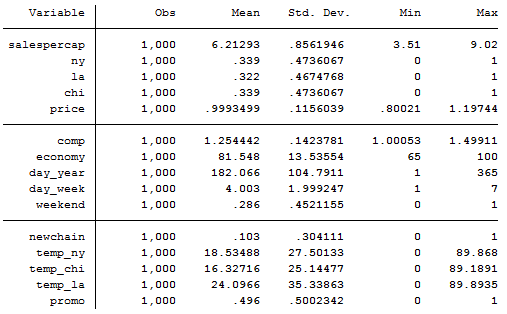
\includegraphics[scale=0.8]{g1.png}\\
Table 1: Summary of the dataset
\end{center}

\begin{center}
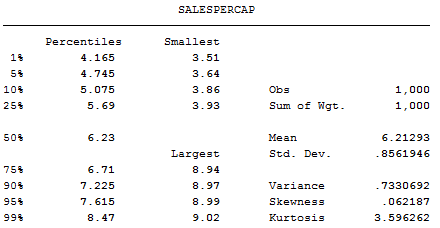
\includegraphics[scale=0.8]{g3.png}\\
Table 2: Interquartile overview of sales per capita
\end{center}

Figure 1 both show the density distribution of the total sales per capita of cups of ice cream and the breakdown of the distribution by {\tt promo}. Distributions seems to be similar and they follow a Normal density distribution. Figure 2 shows a side by side box plot comparison of sales by promo and by non-promo. Figure 3 represents shows the distribution of the sales per capita as a function of ice cream price. 


\begin{center}
 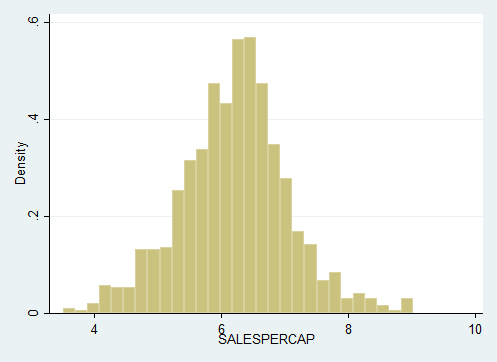
\includegraphics[scale=0.4]{g2.png}
  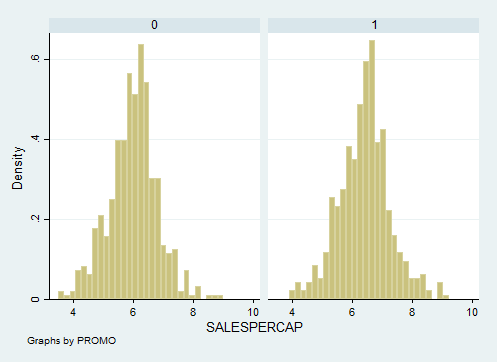
\includegraphics[scale=0.4]{g4.png}\\
Figure 1: Density distribution of sales per capita. Left: Overall sales per capita. Right: Sales per capita by Promo (Marketing campaign)
\end{center}

\begin{center}
  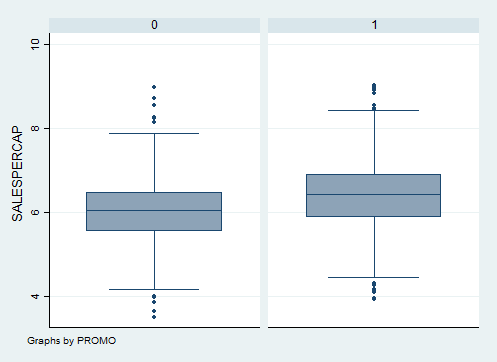
\includegraphics[scale=0.5]{g6.png}\\
Figure 2: Promo Sales seem to perform better than non-promo
\end{center}

\begin{center}
  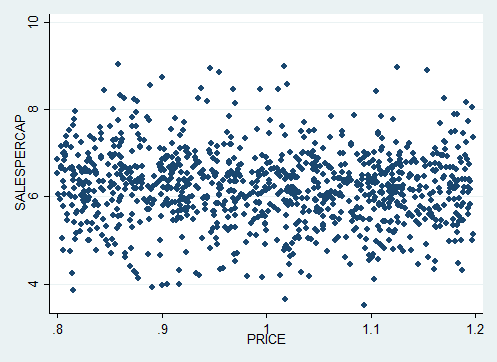
\includegraphics[scale=0.4]{g5.png}\\
Figure 3: Sales per capita as a function of Price
\end{center}


\subsection{Overview by City}

Figure 4 shows the breakdown of the sales per capita distribution by operating city: New York, Los Angeles, and Chicago

\begin{center}
  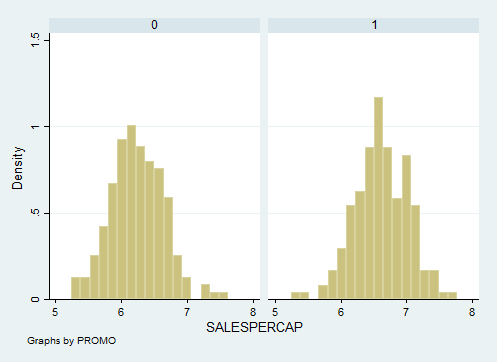
\includegraphics[scale=0.28]{g7_ny.png}
 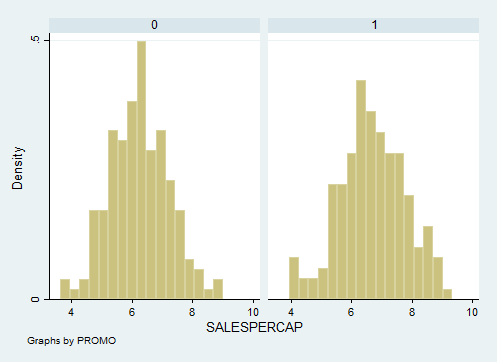
\includegraphics[scale=0.28]{g8_la.png}
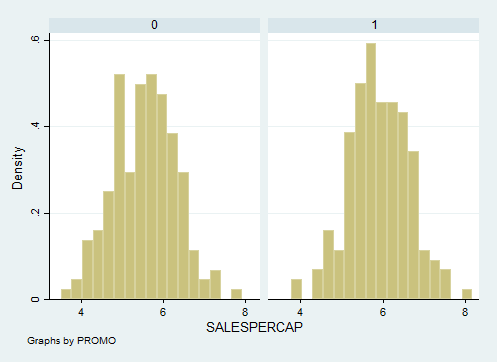
\includegraphics[scale=0.28]{g9_chi.png}\\
Figure 4: Sales per capita distribution by city. Left: New York. Middle: LA. Right: Chicago
\end{center}

%%%%%%%%%%%%%%%%%%%%%%%%%%%%%%%%%%%%%
% 2 Methods
%%%%%%%%%%%%%%%%%%%%%%%%%%%%%%%%%%%%%
\section{Methods}

\subsection{Dataset \& Software}
The dataset analyzed in this paper was taken from the following source\\
 {\tt http://people.fas.harvard.edu/$\sim$mparzen/stat104/icecream2016V1} which contains information about ice cream sales in 2016. The software and version used for the these analyses was Stata/MP 14.0

\subsection{Diagnostic Tests}

In order to account for all the technical problems that could arise in regression, we evaluated Multicollinearity ({\tt vif}), Heteroscedasticity noise ({\tt hettest}), Normality ({\tt sktest}), Outliers (Residuals, Cook's Distance), and Non-linearity ({\tt ovtest}) in our observations 

\subsection{Hypothesis Testing}

The following Null hypothesis were taken into account for diagnostics:
\begin{itemize}
\item $H_0$ for Heteroscedasticity: noise is homoscedastic
\item $H_0$ for Normality: data not normal 
\item $H_0$ for Non-linearity: transformation needed
\end{itemize}

The criteria for statistical significance for Hypothesis testing is P$<0.05$

\subsection{Regression Models}

A total of four regression models were implemented in this paper to predict sales per capita:
\begin{enumerate}
\item Na\"{i}ve Regression 
\item Normal Backward Regression
\item Backward Regression using Adjusted R-Square
\item Backward Regression using AIC
\end{enumerate}

%%%%%%%%%%%%%%%%%%%%%%%%%%%%%%%%%%%%%
% 3 Results
%%%%%%%%%%%%%%%%%%%%%%%%%%%%%%%%%%%%%

\section{Results}

\subsection{Na\"{i}ve Regression Model}
In our first regression model (Model I), we include all variables, we did not perform any diagnostics, transformations, or any modifications to the model, and we use {\tt price} as baseline. Table 3 shows our first regression model

\begin{center}
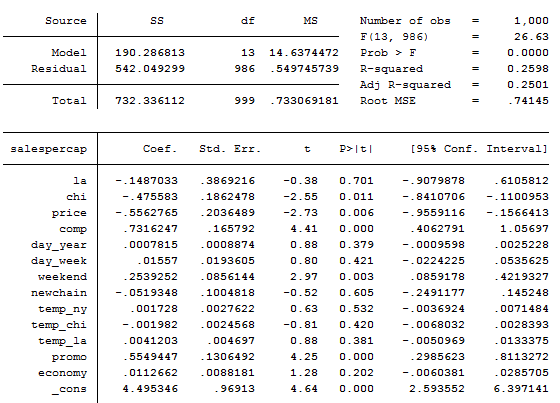
\includegraphics[scale=0.8]{g10.png}\\
Table 3: Model I - The Na\"{i}ve Regression Model
\end{center}

This first model is particularly bad. Both R$^2$ = 0.25 and Adjusted R$^2$ = 0.25 are significantly low, $S_e$ is very high, and the Confidence Intervals describe which variables we do not need in the model: {\tt ny}, {\tt la}, {\tt day\_year}, {\tt day\_week}, {\tt newchain}, {\tt temp\_ny}, {\tt temp\_chi}, {\tt temp\_la}, {\tt economy}  

\subsection{Test for Correlation}

We run a correlation test to identify which variables are highly correlated between each other that might influence our model. Table 4 shows the correlations of all the Xs in our regression model. 

\begin{center}
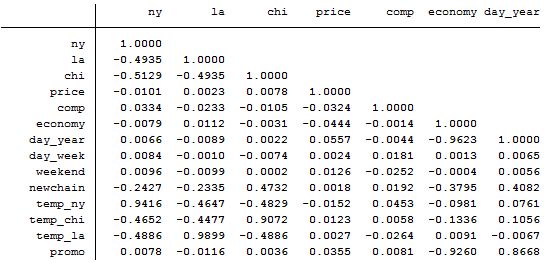
\includegraphics[scale=0.8]{g14.png}\\
Table 4: Correlation across all X variables
\end{center}

Coefficients of $>0.5$ indicate potential Multicollinearity problem.

\subsection{Test for Multicollinearity}

After looking at the correlation of all the Xs in the model, we look for Multicollinearity, i.e., X variables highly related to each other
with the Variance Inflation Factors (VIF) test in Stata. Table 5 shows variables that are highly related to each other

\begin{center}
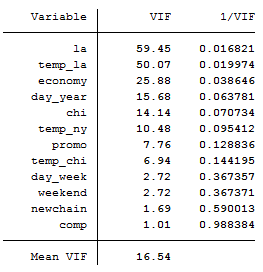
\includegraphics[scale=0.8]{g13.png}\\
Table 5: Results of Multicollinearity Test
\end{center}

Looking at the output, we see that the following variables have a VIF $>$ 10 value: {\tt la}, {\tt temp\_la}, {\tt economy}, {\tt chi}, {\tt day\_year}, and {\tt temp\_ny}. We first, drop {\tt la}, and re-run the model. Second, we drop {\tt ny}, and re-run the model. Third, we drop {\tt economy} and re-run the model. Finally, we drop {\tt chi} and we end up with variables with a VIF $<$ 10 score. 

\subsection{Test for Non-linearity}

Table 6 shows the {\tt ovtest} results for Non-linearity. The p-value is $>0.05$, so we do not need a higher power X in the model. 
\begin{center}
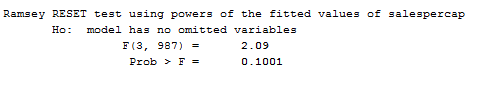
\includegraphics[scale=0.8]{g20.png}\\
Table 6: Non-linearity test results
\end{center}

\subsection{Test for Heteroskedasticity}

Table 7 shows the test results for Heteroskedasticity with {\tt hettest} command

\begin{center}
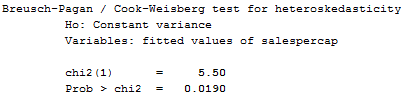
\includegraphics[scale=0.8]{g21.png}\\
Table 7: Heteroskedasticity test results
\end{center}

The null hypothesis for the test is that our residuals have constant variance (i.e.it is homoskedastic). The p-value is $<0.05$, we reject the null hypothesis and conclude the residuals are heteroskedastic.

\subsection{Test for Normality \& Outliers }
 
Testing {\tt sktest res} we find a P-value of 0.0001, so we reject the Null and conclude that the residual {\tt res} is not normally distributed. We evaluate standard residual {\tt sres} and we drop outliers with {\tt sres} values smaller than -2.0 and bigger than 2.0. This results in a new {\tt sktest res} p-value of 0.3102 hence our data is now normally distributed. Figure 5 and Figure 6 show the results of the normality tests without outliers. 

\begin{center}
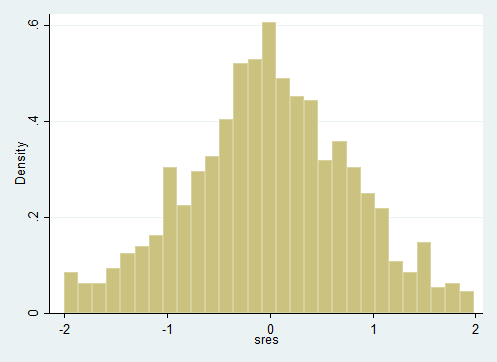
\includegraphics[scale=0.4]{g16.png}\\
Figure 5: Density distribution of Standard Residual
\end{center}

\begin{center}
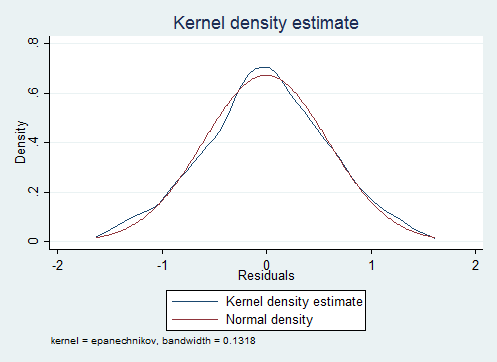
\includegraphics[scale=0.4]{g15.png}\\
Figure 6: Normality Test on Residuals
\end{center}

\subsection{Obtaining Residuals}

We check the residuals with {\tt rvfplot} in Figure 7 to check if there is a weird distribution of the data
\begin{center}
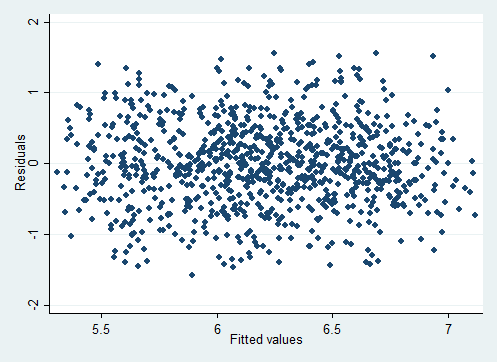
\includegraphics[scale=0.4]{g17.png}\\
Figure 7: Residual plot distribution
\end{center}

The data looks randomly distributed and no weird shape. 

\subsection{Cook's Distance \& Outliers}

A Cook's Distance is calculated for each row in our dataset, we see extreme values of Cook's Distance which indicate points that are probably influential in Figure 8. 

\begin{center}
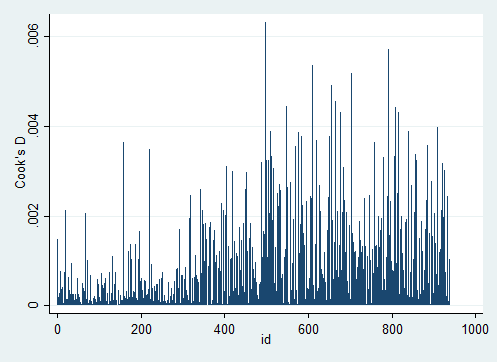
\includegraphics[scale=0.5]{g18.png}\\
Figure 8: Result of Cook's Distance
\end{center}

We drop observations (outliers) with Cook's Distance $D>0.005$

\subsection{Regular Backward Regression}

We implement at regular backward regression (throwing out highest p-value one at a time) with the following X variables: {\tt price}, {\tt comp}, {\tt day\_year}, {\tt day\_week}, {\tt weekend}, {\tt newchain}, {\tt temp\_ny}, {\tt temp\_chi}, {\tt temp\_la}, and {\tt promo}. Table 8 shows the new model (Model II) with price as baseline

\begin{center}
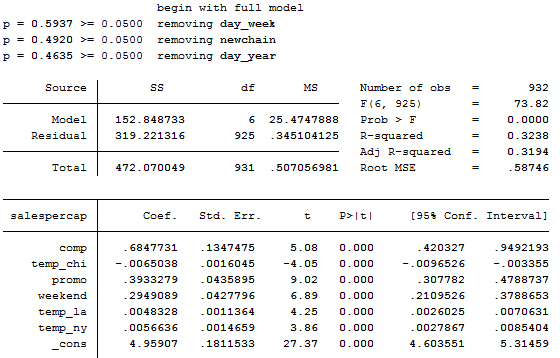
\includegraphics[scale=0.8]{g19.png}\\
Table 8: Model II - Regular Backward Regression Model 
\end{center}

From this result, we don't need the variables {\tt day\_week}, {\tt newchain}, and {\tt day\_year} in the model.

\subsection{Backward Regression using Adjusted R-Square}

Our next model implements {\tt backward r2adj} and optimizes for Adjusted R-Square. Table 9 shows the results of our next model (Model III). 

\begin{center}
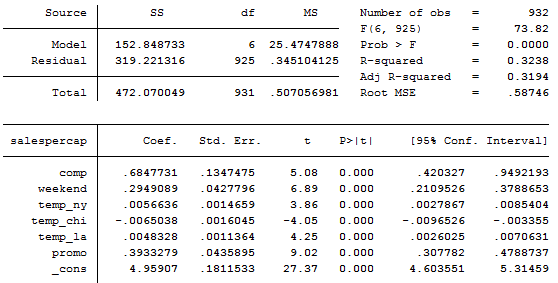
\includegraphics[scale=0.8]{g22.png}\\
Table 9: Model III - Backward using Adjusted R-Square Model
\end{center}

\subsection{Backward Regression using AIC}

Our final  model implements {\tt backward aic} and optimizes for Adjusted R-Square. Table 10 shows the results of our final model (Model IV). 

\begin{center}
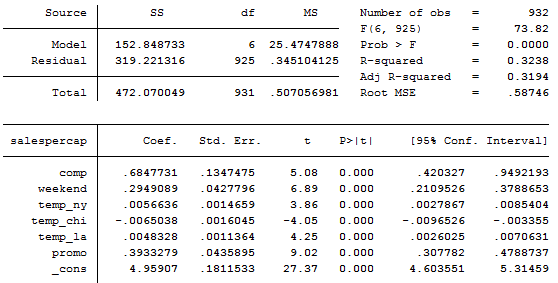
\includegraphics[scale=0.8]{g22.png}\\
Table 10: Model IV - Backward Regression using AIC Model
\end{center}


\section{Conclusion \& Discussion}

We determine, using different diagnostic tools, what effects are contained in the dataset help to explain CrimsonCream Inc ice cream sales. We run 4 different regression models and the results are show in Table 11

\newpage

\begin{center}
\begin{tabular}{|c|c|c|c|c|}
\hline
{\bf Model} & {\bf Regression Type} & {\bf R$^2$} & {\bf Adjusted R$^2$} & {\bf $S_e$} \\
\hline
Model I & Na\"{i}ve &  0.2598 & 0.2501 & 0.7414\\
Model II & Normal Backward &0.3238 & 0.3194 & 0.5874 \\
Model III & Backward Adjusted R$^2$ & 0.3238 & 0.3194 & 0.5874 \\
Model IV & Backward AIC & 0.3238 & 0.3194 & 0.48746 \\
\hline
\end{tabular}\\
Table 11: Summary of Regression Models
\end{center}

Model IV has the lowest $S_e$ value, hence we present the equation that adequately describes the sales per capita with price as baseline:

\begin{center}
{\tt salespercap = 0.684*comp + 0.393*promo + 0.295*weekend - 0.006*temp\_chi + 0.005*temp\_la + 0.005*temp\_ny + 4.95}
\end{center}

We observe that the Adjusted R-Square value of Model IV higher and the value of $S_e$ is lower compared to Model I which indicates this is a better model than our na\"{i}ve regression model. Looking at the $S_e$, if we use this model to predict the core price of ice cream sales, we would be at +/- 0.96 units with 95\% confidence. \\

This formula takes on two forms for {\tt promo = 0,1}.
\begin{itemize}
\item For {\tt promo = 0}
\begin{center}
 y = {\tt 0.684*comp + 0.295*weekend - 0.006*temp\_chi + 0.005*temp\_la + 0.005*temp\_ny + 4.95}
\end{center}
\item For {\tt promo = 1}
\begin{center}
{\tt y = 0.684*comp + 0.295*weekend - 0.006*temp\_chi + 0.005*temp\_la + 0.005*temp\_ny + 5.34}
\end{center}
\end{itemize}

For a given day ({\tt weekend} = 0,1), the sales on promo ({\tt promo} = 1), have on average sales per capita 0.393 points higher than those not running on promo ({\tt promo} = 0). This shows that the promotional Marketing campaign worked. There was more sales when the campaign was running. 

\begin{thebibliography}{9}

\bibitem{lamport94}
StataCorp. 2015. Stata Statistical Software: Release 14. College Station, TX: StataCorp LP.

\bibitem{lamport94} 
STAT 104 Quantitative Methods for Economists. 2016. Dataset taken from http://people.fas.harvard.edu/$\sim$mparzen/stat104/icecream2016V1

\end{thebibliography}


\end{document}